
\section{Données et résultats}\label{sec:resultats}

\subsection{Données}

Les relevés donnent, minute par minute, le nombre de vélos mécaniques, de vélos électriques et de bornes libres de chaque station. Ils proviennent des données temps réel de Vélib' Métropole, consultées sur le site \texttt{velib.nocle.fr}. Le tableau~\ref{tab:donnees} résume les séries~: quatre jours ouvrés consécutifs à Gare de Lyon ($C=45$) et deux à Nation ($C=36$), représentés sur la figure~\ref{fig:donnees}, puis une journée de week-end, du samedi 23 mai 21~h au dimanche 24 mai 21~h, pour quatre stations. Les minutes manquantes, environ une par heure, sont complétées par la dernière valeur connue~; les doublons et deux erreurs de saisie de la capacité sont écartés. L'état $X_t$ est la somme des vélos mécaniques et électriques. Une ou deux bornes sont souvent hors service, si bien que $C-X_t$ dépasse le nombre de bornes libres.

\begin{figure*}[t]
\centering
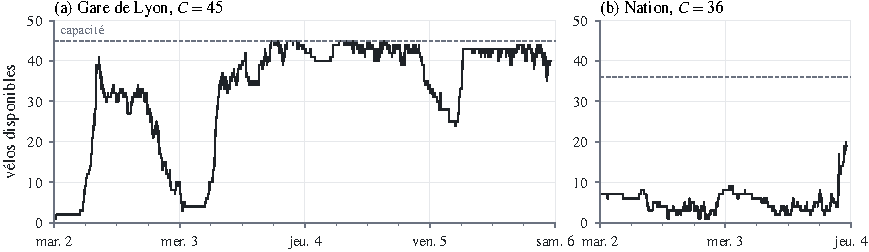
\includegraphics[width=\textwidth]{figures/fig_donnees.pdf}
\caption{Nombre de vélos disponibles, relevé chaque minute. (a)~Gare de Lyon, du mardi 2 au vendredi 5 juin 2026~; (b)~Nation, 2 et 3 juin. Tirets~: capacité.}\label{fig:donnees}
\end{figure*}

\begin{table}[t]
\centering\small
\caption{Séries utilisées. $\Nu$, $\Nd$~: dépôts et retraits comptés~; dernières colonnes~: minutes passées pleine et vide.}\label{tab:donnees}
\setlength{\tabcolsep}{4pt}
\begin{tabular}{@{}lrrrrrr@{}}
\toprule
Station & $C$ & heures & $\Nu$ & $\Nd$ & pleine & vide\\
\midrule
@@TAB_DONNEES@@
\bottomrule
\end{tabular}
\end{table}

\subsection{Le régime stationnaire n'est pas observé}\label{sec:nonstationnaire}

Le TIPE ajustait le modèle à taux constants sur la journée du mardi, de 9~h à 19~h. On obtient $\hat\lambda=@@lam919@@$ $[@@lam919a@@\,;\,@@lam919b@@]$ et $\hat\mu=@@mu919@@$ $[@@mu919a@@\,;\,@@mu919b@@]\hr$, soit $\hat\rho=@@rho919@@$ $[@@rho919a@@\,;\,@@rho919b@@]$ (tableau~\ref{tab:fenetres}). La loi stationnaire place alors la station près de $0$~: $\EE_\pi[X]=@@estat919@@$, alors que la station contient en moyenne @@emp919@@~vélos sur la fenêtre. La distance en variation totale entre $\pi$ et l'occupation observée vaut @@vt919@@ (fig.~\ref{fig:stationnaire}a). Le TIPE concluait à l'échec du modèle.

C'est l'approximation stationnaire qui échoue, pas le modèle. La loi de $X_t$ issue de l'état observé à 9~h ($X=@@x0919@@$), calculée avec les mêmes taux, contient la trajectoire dans sa bande à 90~\% pendant @@couv919@@~\% des minutes (fig.~\ref{fig:stationnaire}b). Le temps de relaxation vaut @@relax919@@~h et le temps de mélange @@mel919@@~h~: sur une fenêtre de 10~h, la chaîne n'a pas le temps d'oublier son état initial. À Nation, sur la même fenêtre, $\trel=@@relaxnat@@$~h et $\tmel=@@melnat@@$~h.

\begin{figure}[t]
\centering
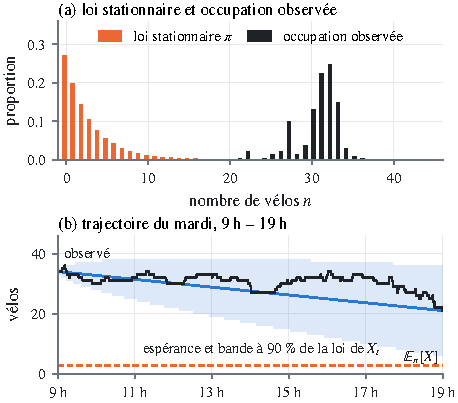
\includegraphics[width=\columnwidth]{figures/fig_stationnaire.pdf}
\caption{Gare de Lyon, mardi 2 juin, 9~h--19~h. (a)~Loi stationnaire du modèle ajusté ($\hat\rho=@@rho919@@$) et occupation observée. (b)~Trajectoire observée, espérance et bande à 90~\% de la loi de $X_t$ issue de l'état observé à 9~h, avec les mêmes taux.}\label{fig:stationnaire}
\end{figure}

\begin{table}[t]
\centering\small
\caption{Estimations sur quelques fenêtres, avec l'intervalle de confiance à 95~\% de $\rho$ (section~\ref{sec:estimation}). Taux en $\mathrm{h}^{-1}$.}\label{tab:fenetres}
\setlength{\tabcolsep}{3.5pt}
\begin{tabular}{@{}lrrrrl@{}}
\toprule
Fenêtre & $\Nu$ & $\Nd$ & $\hat\lambda$ & $\hat\mu$ & $\hat\rho$ \ [IC 95~\%]\\
\midrule
@@TAB_FENETRES@@
\bottomrule
\end{tabular}
\end{table}

\subsection{Saisonnalité intrajournalière}\label{sec:saison}

On découpe la journée en douze créneaux de 2~h et on estime $(\lambda_k,\mu_k)$ en regroupant les quatre jours ouvrés (fig.~\ref{fig:forcage}, tableau~\ref{tab:creneaux}). La pointe du matin, de 6~h à 8~h, compte @@nd_pointe@@ dépôts pour @@np_pointe@@ retraits~: $\hat\rho\approx@@rho_pointe@@$. La station reçoit alors les vélos des usagers qui rejoignent la gare ou les bureaux du quartier. Le dimanche 24 mai, cette pointe disparaît ($\hat\lambda=@@lam_dim68@@\hr$ de 6~h à 8~h) et les dépôts culminent de 10~h à 12~h ($\hat\lambda=@@lam_dim1012@@\hr$).

Les tests du rapport de vraisemblance (section~\ref{sec:rv}) donnent~:
\begin{itemize}
\item taux constants sur la journée~: $W=@@w_dj@@$ (11 degrés de liberté, $p=@@p_dj@@$) pour les dépôts, $W=@@w_pj@@$ ($p=@@p_pj@@$) pour les retraits~;
\item taux constants de 8~h à 20~h~: $p=@@p_d820@@$ et $p=@@p_p820@@$~;
\item même profil chaque jour, créneau par créneau~: $p=@@p_dej@@$ et $p=@@p_pej@@$.
\end{itemize}
Les taux varient au cours de la journée, et le profil lui-même varie d'un jour à l'autre. Le second point annonce des bandes de prédiction trop étroites hors échantillon~: des taux moyens ne captent pas la variabilité entre jours.

Tous les temps de mélange du tableau~\ref{tab:creneaux} dépassent @@melmin@@~h, soit plus du double de la durée d'un créneau~; de 8~h à 22~h, ils sont compris entre @@meljour_a@@ et @@meljour_b@@~h. La loi stationnaire d'un créneau n'est donc jamais atteinte. Seule la loi transitoire, propagée de créneau en créneau, a un sens. La figure~\ref{fig:melange} illustre les deux régimes de la remarque~\ref{rem:melange}. De 8~h à 10~h ($\hat\rho\approx1$), la convergence est lente et diffusive. De 6~h à 8~h ($\hat\rho\approx@@rho_pointe@@$), $1/\gamma$ ne vaut que @@relax_pointe_min@@~min, mais la chaîne issue de $0$ reste à distance $1$ de $\pi$ pendant plusieurs heures, le temps de traverser la station.

\begin{figure}[t]
\centering
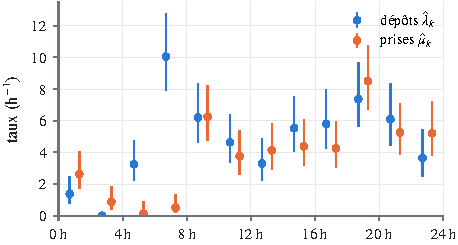
\includegraphics[width=\columnwidth]{figures/fig_forcage.pdf}
\caption{Taux de dépôt et de retrait par créneau de 2~h, Gare de Lyon, quatre jours ouvrés regroupés, avec intervalles de confiance à 95~\%.}\label{fig:forcage}
\end{figure}

\begin{table}[t]
\centering\small
\caption{Taux par créneau (en $\mathrm{h}^{-1}$), temps de relaxation et temps de mélange de la chaîne à taux constants correspondante, en heures. Aucun dépôt n'est observé de 2~h à 4~h.}\label{tab:creneaux}
\setlength{\tabcolsep}{4.5pt}
\begin{tabular}{@{}lrrrrr@{}}
\toprule
Créneau & $\hat\lambda_k$ & $\hat\mu_k$ & $\hat\rho_k$ & $\trel$ & $\tmel$\\
\midrule
@@TAB_CRENEAUX@@
\bottomrule
\end{tabular}
\end{table}

\begin{figure}[t]
\centering
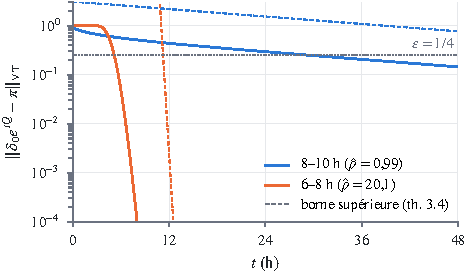
\includegraphics[width=\columnwidth]{figures/fig_melange.pdf}
\caption{Distance à l'équilibre depuis la station vide, avec les taux de deux créneaux de Gare de Lyon. Tirets~: majoration du théorème~\ref{thm:vitesse}~; pointillés~: seuil $1/4$ qui définit $\tmel$.}\label{fig:melange}
\end{figure}

\subsection{Prévision hors échantillon}\label{sec:prevision}

\paragraph{Protocole} Pour prévoir un jour, on estime les taux par créneau sur les autres jours ouvrés (validation croisée \og un jour exclu\fg{}), et on calcule la loi exacte de $X_t$ à partir de l'état observé au début de l'horizon. On mesure l'écart absolu moyen (EAM) entre l'espérance et la trajectoire, et la couverture de la bande à 90~\%, c'est-à-dire la fraction des minutes où la trajectoire est dans la bande.

\paragraph{Horizon 2~h} Sur les @@n2h@@ créneaux de Gare de Lyon, la bande couvre @@couv2h@@~\% des minutes, pour 90~\% visés. En fin de créneau, la valeur observée sort de la bande @@hors2h@@ fois, contre @@att2h@@ attendues (test binomial, $p=@@pbin2h@@$). L'erreur quadratique moyenne en fin de créneau vaut @@rmse2h@@~vélos, contre @@rmsenaif2h@@ pour la prévision naïve \og pas de changement\fg{}. À Nation, station peu active, la couverture atteint @@couv2hnat@@~\%, mais la prévision naïve fait mieux (@@rmsenaif2hnat@@ contre @@rmse2hnat@@~vélos). Les trois créneaux les plus mal couverts, avec moins de 10~\% des minutes dans la bande, sont des nuits ou des soirées où la station perd des vélos, ce que les autres jours ne laissaient pas prévoir~: le mardi de 20~h à 22~h, elle passe de @@soir_x0@@ à @@soir_x1@@~vélos alors que l'espérance prévue monte à @@soir_prev@@ (fig.~\ref{fig:court}b).

\begin{figure}[t]
\centering
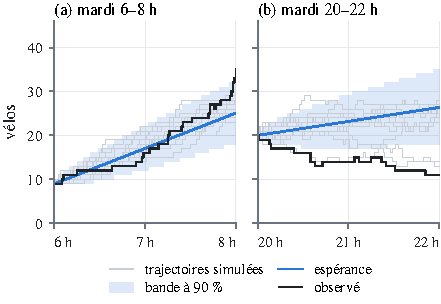
\includegraphics[width=\columnwidth]{figures/fig_court.pdf}
\caption{Prévision à 2~h hors échantillon, Gare de Lyon, mardi 2 juin~: taux estimés sur les trois autres jours, état initial observé. (a)~Pointe du matin~; (b)~soirée atypique.}\label{fig:court}
\end{figure}

\paragraph{Horizon 24~h} Le tableau~\ref{tab:jour} compare trois modèles partant de l'état observé à minuit~: taux constants et taux par créneaux, estimés hors échantillon, puis taux par créneaux estimés sur le jour même, en échantillon, qui donnent une borne inférieure de l'erreur. À Gare de Lyon, les créneaux réduisent l'EAM moyen de @@eam24c@@ à @@eam24k@@~vélos et portent la couverture de @@couv24c@@ à @@couv24k@@~\%. L'écart restant avec le modèle en échantillon (@@eam24i@@~vélos) mesure la variabilité d'un jour à l'autre. Le mardi et le mercredi, qui démarrent presque vides, sont les plus mal prévus (fig.~\ref{fig:jour}).

\begin{table}[t]
\centering\small
\caption{Prévision à 24~h depuis l'état $X_0$ observé à minuit~: EAM en vélos et, entre parenthèses, couverture de la bande à 90~\% en pourcentage.}\label{tab:jour}
\setlength{\tabcolsep}{4pt}
\begin{tabular}{@{}lrlll@{}}
\toprule
Jour & $X_0$ & constants & créneaux & jour même\\
\midrule
@@TAB_24H@@
\bottomrule
\end{tabular}
\end{table}

\begin{figure*}[t]
\centering
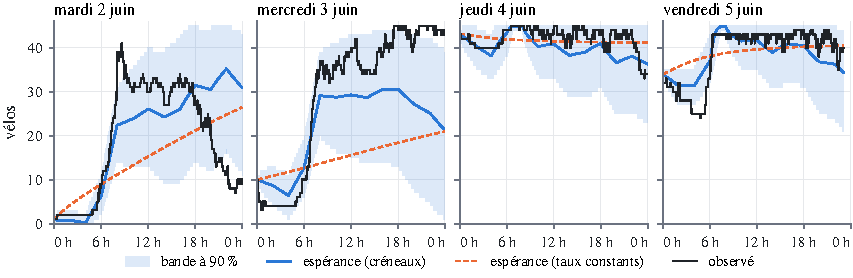
\includegraphics[width=\textwidth]{figures/fig_jour.pdf}
\caption{Prévision à 24~h hors échantillon depuis l'état observé à minuit, Gare de Lyon. Bleu~: taux par créneaux estimés sur les trois autres jours (espérance et bande à 90~\%)~; tirets orange~: taux constants.}\label{fig:jour}
\end{figure*}

\subsection{Régime périodique}\label{sec:regime}

En répétant chaque jour le profil moyen des taux, on se place dans le cadre de la proposition~\ref{prop:periodique}. La matrice $M$, produit des douze exponentielles, vérifie $|\lambda_2(M)|=@@vp2@@$ et $\delta(M)=@@doeblin@@$~: l'écart à la loi invariante est divisé par environ @@inv_vp2@@ chaque jour. La loi invariante $\nu$ à minuit a pour moyenne @@moyminuit@@~vélos et pour bande à 90~\% $[@@q05minuit@@\,;\,@@q95minuit@@]$~; sous $\nu$, $\PP(X\leq10)=@@pinf10@@$. Le vélo unique du mardi 0~h et les 10 vélos du mercredi 0~h sont donc atypiques. Ils signalent une intervention extérieure, typiquement un camion de régulation, que le modèle ne contient pas.

La figure~\ref{fig:periodique} prolonge la prévision du mardi 0~h sur quatre jours. La distance en variation totale à $\nu$ passe de @@vt24@@ à 24~h à @@vt48@@ à 48~h, puis @@vt72@@ à 72~h. La trajectoire reste dans la bande @@couv4j@@~\% du temps. La \og dérive\fg{} d'un jour à l'autre relevée dans le TIPE (le forçage se répète, pas la réponse) est ce régime transitoire~: la réponse se répète une fois l'état initial oublié, soit après deux jours environ.

\begin{figure*}[t]
\centering
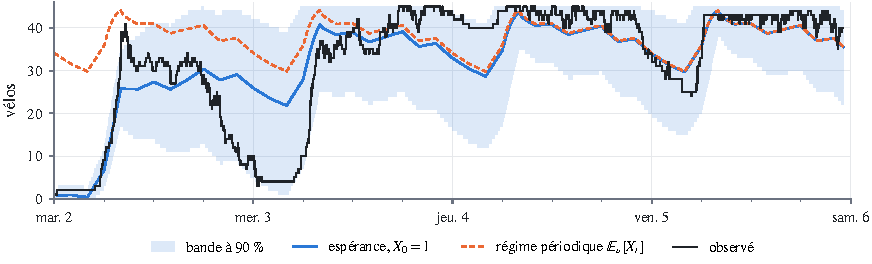
\includegraphics[width=\textwidth]{figures/fig_periodique.pdf}
\caption{Prévision sur quatre jours depuis le mardi 0~h ($X_0=1$), avec le profil moyen des taux répété chaque jour. Tirets~: espérance dans le régime périodique.}\label{fig:periodique}
\end{figure*}

\paragraph{Qualité de service} Dans le régime périodique, la station est pleine @@tplein@@~\% du temps et refuse @@deprefus@@~\% des dépôts, fraction pondérée par l'intensité des dépôts (propriété PASTA)~; elle n'est presque jamais vide (@@tvide@@~\% du temps). Sur @@nsim@@ journées simulées à partir de $\nu$, la station sature au moins une fois dans @@psat@@~\% des cas~; le temps quotidien passé à saturation a pour médiane @@dmed@@~min et pour intervalle à 90~\% $[@@dq05@@\,;\,@@dq95@@]$~min. Les valeurs observées du mardi au vendredi sont @@dobs@@~min~; seule la première, après un départ presque vide, sort de l'intervalle.

\subsection{Écarts à l'hypothèse poissonnienne}\label{sec:poisson}

\paragraph{Arrivées groupées} Sous (H1), avec les taux du créneau, la variation nette d'une minute suit une loi de Skellam, différence de deux lois de Poisson indépendantes. Le tableau~\ref{tab:lots} compare le nombre de minutes où la station gagne, ou perd, au moins deux vélos au nombre attendu. Sur l'ensemble des séries, on observe @@lots_obs@@ telles minutes pour @@lots_att@@ attendues, soit un facteur @@lots_rapport@@ ($p=@@lots_p@@$ sous l'approximation de Poisson). Une partie des usagers arrive en groupe, par exemple à la descente d'un train à Gare de Lyon. Un processus de Poisson composé ou un processus de Hawkes \cite{BMM15} rendrait compte de cette surdispersion.

\begin{table}[t]
\centering\small
\caption{Minutes avec une hausse ($\Delta\geq2$) ou une baisse ($\Delta\leq-2$) d'au moins deux vélos~: nombre observé et nombre attendu sous (H1) avec les taux de chaque créneau.}\label{tab:lots}
\setlength{\tabcolsep}{4pt}
\begin{tabular}{@{}lrrrr@{}}
\toprule
& \multicolumn{2}{c}{$\Delta\geq2$} & \multicolumn{2}{c}{$\Delta\leq-2$}\\
\cmidrule(lr){2-3}\cmidrule(l){4-5}
Série & obs. & att. & obs. & att.\\
\midrule
@@TAB_LOTS@@
\bottomrule
\end{tabular}
\end{table}

\paragraph{Régulation} Certaines variations sont incompatibles avec le modèle. À Nation, le mercredi 3 juin entre 21~h~36 et 21~h~46, la station passe de @@nat_x0@@ à @@nat_x1@@~vélos. Avec le taux de dépôt de la veille sur le même créneau ($@@nat_taux_veille@@\hr$), la probabilité d'au moins @@nat_hausse@@ dépôts en 10~min est de l'ordre de $@@nat_p_veille@@$. À Gare de Lyon, le dimanche 24 mai à 20~h~54, la station perd @@gdl_saut@@~vélos en une minute ($p\approx@@gdl_p_minute@@$ avec le taux de retrait du créneau précédent). Ce sont des camions de l'opérateur. La régulation est un contrôle exogène~: le modèle complet est une chaîne contrôlée, avec des sauts imposés à des instants choisis par l'opérateur.

\section{Discussion~: lecture en finance quantitative}\label{sec:discussion}

\paragraph{Files d'ordres} Dans le modèle de Cont, Stoikov et Talreja \cite{CST10}, la quantité d'ordres à chaque niveau de prix est un processus de naissance et de mort~: les ordres limites l'alimentent, les ordres au marché et les annulations la vident. La probabilité que le meilleur prix monte est celle qu'une file se vide avant une autre, un problème de premier passage du type du corollaire~\ref{cor:ruine}, résolu par transformée de Laplace. Cont et de Larrard \cite{CdL13} en tirent une limite diffusive du prix. Huang, Lehalle et Rosenbaum \cite{HLR15} font dépendre les intensités de la taille de la file. Pour une station, l'analogue serait des taux $\lambda(n)$ et $\mu(n)$ dépendant de $n$, par exemple si l'application détourne les usagers des stations presque vides. La loi stationnaire reste explicite par équilibre détaillé~: $\pi_n\propto\prod_{j=0}^{n-1}\lambda(j)/\mu(j+1)$.

\paragraph{Risque de crédit} Jarrow, Lando et Turnbull \cite{JLT97} décrivent la notation d'un émetteur par une chaîne de Markov à temps continu dont le défaut est l'état absorbant. Lando et Skødeberg \cite{LS02} estiment le générateur à partir des dates exactes de migration, avec l'estimateur de la proposition~\ref{prop:emv}~; l'estimateur en temps continu attribue une probabilité non nulle à des transitions rares jamais observées sur un an. La remarque de la section~\ref{sec:minute} sur la compensation en est la version à la minute~: l'échantillonnage discret masque les allers-retours, pas la dérive.

\paragraph{Saisonnalité et agrégats} L'intensité des transactions suit un profil intrajournalier marqué, que l'on traite comme ici par une intensité déterministe par morceaux avant de modéliser le résidu. Les arrivées groupées (section~\ref{sec:poisson}) et la variabilité entre jours (section~\ref{sec:saison}) ont pour analogues les agrégats d'ordres que décrivent les processus de Hawkes \cite{BMM15}.

\paragraph{Validation} Le protocole de la section~\ref{sec:prevision} est celui d'un backtest~: paramètres estimés sur une période, prévision évaluée sur une autre, couverture comparée au niveau nominal comme pour une VaR \cite{Kup95}. Les minutes successives étant très corrélées, le test porte sur les valeurs de fin de créneau.

\paragraph{Limites} Les données couvrent six jours~; les taux d'un créneau reposent sur quatre jours au plus, d'où des intervalles larges (fig.~\ref{fig:forcage}). Chaque station est traitée isolément, alors que les dépôts d'une station sont les retraits d'une autre. Les camions de régulation ne sont pas modélisés.

\section{Conclusion}

Une station Vélib' se décrit bien par une chaîne de naissance et de mort à taux constants par créneaux, à condition de calculer la loi transitoire et non la loi stationnaire. Les temps de mélange, de @@melmin_ent@@ à @@melmax_ent@@~h, dépassent la durée pendant laquelle les taux restent constants~: la loi stationnaire d'un créneau n'est jamais observée. L'objet pertinent est le régime périodique, atteint en deux jours environ. Hors échantillon, le modèle prévoit l'occupation à 2~h avec une couverture proche du niveau visé~; à 24~h, la variabilité entre jours domine. Les écarts restants, arrivées groupées et camions de régulation, indiquent les extensions naturelles~: processus de Poisson composé ou de Hawkes, intensités dépendant de l'état, contrôle optimal de la régulation.

\appendix
\section{Code}\label{sec:code}

Le module \texttt{velib.py} contient les fonctions de simulation, d'estimation et de calcul exact. Les scripts fournis avec l'article (lecture des relevés, calculs, figures) s'appuient sur ce module, sur \texttt{numpy}, \texttt{scipy} et \texttt{matplotlib}.

\begin{lstlisting}[style=py]
@@CODE@@
\end{lstlisting}

\begin{thebibliography}{STGH18}
\small\sloppy\NoAutoSpacing
\setlength{\itemsep}{1pt}
\bibitem[Alb62]{Alb62} A.~Albert. Estimating the infinitesimal generator of a continuous time, finite state Markov process. \emph{Ann. Math. Statist.}, 33(2):727--753, 1962.
\bibitem[Bil61]{Bil61} P.~Billingsley. \emph{Statistical Inference for Markov Processes}. University of Chicago Press, 1961.
\bibitem[BMM15]{BMM15} E.~Bacry, I.~Mastromatteo, J.-F.~Muzy. Hawkes processes in finance. \emph{Market Microstructure and Liquidity}, 1(1):1550005, 2015.
\bibitem[Bré99]{Bre99} P.~Brémaud. \emph{Markov Chains: Gibbs Fields, Monte Carlo Simulation, and Queues}. Springer, 1999.
\bibitem[CdL13]{CdL13} R.~Cont, A.~de Larrard. Price dynamics in a Markovian limit order market. \emph{SIAM J. Financial Math.}, 4(1):1--25, 2013.
\bibitem[CST10]{CST10} R.~Cont, S.~Stoikov, R.~Talreja. A stochastic model for order book dynamics. \emph{Oper. Res.}, 58(3):549--563, 2010.
\bibitem[DVJ03]{DVJ03} D.~J.~Daley, D.~Vere-Jones. \emph{An Introduction to the Theory of Point Processes}, vol.~I. Springer, 2\textsuperscript{e}~éd., 2003.
\bibitem[FG16]{FG16} C.~Fricker, N.~Gast. Incentives and redistribution in homogeneous bike-sharing systems with stations of finite capacity. \emph{EURO J. Transp. Logist.}, 5(3):261--291, 2016.
\bibitem[Gil77]{Gil77} D.~T.~Gillespie. Exact stochastic simulation of coupled chemical reactions. \emph{J. Phys. Chem.}, 81(25):2340--2361, 1977.
\bibitem[Guy07]{Guy07} A.~Guyader. \emph{Processus markoviens de sauts}. Notes de cours, master de statistique, Université Rennes~2, 2006--2007.
\bibitem[HLR15]{HLR15} W.~Huang, C.-A.~Lehalle, M.~Rosenbaum. Simulating and analyzing order book data: the queue-reactive model. \emph{J. Amer. Statist. Assoc.}, 110(509):107--122, 2015.
\bibitem[JLT97]{JLT97} R.~A.~Jarrow, D.~Lando, S.~M.~Turnbull. A Markov model for the term structure of credit risk spreads. \emph{Rev. Financ. Stud.}, 10(2):481--523, 1997.
\bibitem[JP04]{JP04} J.~Jacod, P.~Protter. \emph{Probability Essentials}. Springer, 2\textsuperscript{e}~éd., 2004.
\bibitem[Kup95]{Kup95} P.~H.~Kupiec. Techniques for verifying the accuracy of risk measurement models. \emph{J. Derivatives}, 3(2):73--84, 1995.
\bibitem[LP17]{LP17} D.~A.~Levin, Y.~Peres, avec E.~L.~Wilmer. \emph{Markov Chains and Mixing Times}. American Mathematical Society, 2\textsuperscript{e}~éd., 2017.
\bibitem[LS02]{LS02} D.~Lando, T.~M.~Skødeberg. Analyzing rating transitions and rating drift with continuous observations. \emph{J. Bank. Finance}, 26(2--3):423--444, 2002.
\bibitem[Nor97]{Nor97} J.~R.~Norris. \emph{Markov Chains}. Cambridge University Press, 1997.
\bibitem[RK13]{RK13} T.~Raviv, O.~Kolka. Optimal inventory management of a bike-sharing station. \emph{IIE Trans.}, 45(10):1077--1093, 2013.
\bibitem[SHH17]{SHH17} J.~Schuijbroek, R.~C.~Hampshire, W.-J.~van Hoeve. Inventory rebalancing and vehicle routing in bike sharing systems. \emph{European J. Oper. Res.}, 257(3):992--1004, 2017.
\bibitem[STGH18]{STGH18} J.~F.~Shortle, J.~M.~Thompson, D.~Gross, C.~M.~Harris. \emph{Fundamentals of Queueing Theory}. Wiley, 5\textsuperscript{e}~éd., 2018.
\bibitem[Wol82]{Wol82} R.~W.~Wolff. Poisson arrivals see time averages. \emph{Oper. Res.}, 30(2):223--231, 1982.
\end{thebibliography}

\end{document}
